\section{Dreiachsiger Spannungszustand\label{spannung:section:Dreiachsiger_Spannungszustand}}
\rhead{Proportionalität Spannung-Dehnung}
Wie im Kapitel Spannungsausbreitung beschrieben herrscht in jedem Punkt ein anderer Spannungszustand.
Um die Spannung im Boden genauer untersuchen zu können für man einen infinitesimalen Würfel ein.
\begin{figure}
	\centering
	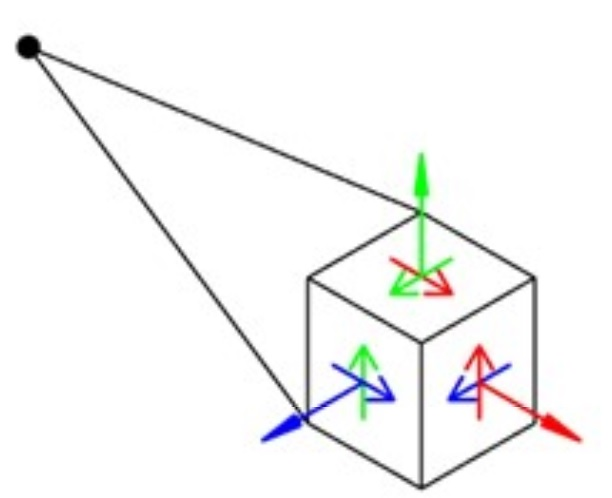
\includegraphics[width=0.5\linewidth,keepaspectratio]{papers/spannung/Grafiken/infinitesimalerWuerfel.jpg}
	\caption{Infinitesimaler Würfel}
	\label{fig:infintesimaler-wurfel}
\end{figure}

Sobald eine Kraft von oben wirkt hat man auch Kräfte die seitlich wirken.

An diesem infinitesimalen Würfel hat man ein räumliches Koordinatensystem, die Achsen $(1,2,3)$.
Jede dieser 6 Flächen dieses Würfels hat damit 3 Pfeile.
Geschrieben werden diese mit $\sigma$ mit jeweils zwei Indizes gibt.
Die Indizes geben uns an, in welche Richtung der Pfeil zeigt.
Der erste Index ist die Achse auf welcher man sich befindet.
Der zweite Index gibt an, in welche Richtung der Pfeil zeigt.
Zur Notation wird die Voigt'sche Notation benutzt. Das sieht wie folgt aus:

\[
\overline{\sigma}
=
\begin{pmatrix}
	\sigma_{11} & \sigma_{12} & \sigma_{13} \\ 
	\sigma_{21} & \sigma_{22} & \sigma_{23} \\
	\sigma_{31} & \sigma_{32} & \sigma_{33}
\end{pmatrix}
=
\begin{pmatrix}
	\sigma_{11} & \sigma_{12} & \sigma_{13} \\ 
	& \sigma_{22} & \sigma_{23} \\
	sym &  & \sigma_{33} \\ 
\end{pmatrix}
\Rightarrow
\overrightarrow{\sigma}
=
\begin{pmatrix}
  \sigma_{11}\\
	\sigma_{22}\\
	\sigma_{33}\\
	\sigma_{23}\\
	\sigma_{13}\\
	\sigma_{12}
\end{pmatrix}
\]

Voigt'sche Notation besagt, dass man diesen Spannungstensor als Vektor aufschreiben darf.
Die Reihenfolge folgt der Regel von Ecke links oben, diagonal zur Ecke rechts unten.
Danach ist noch $\sigma_{23}$, $\sigma_{13}$ und $\sigma_{12}$ aufzuschreiben.

Eine weitere Besonderheit ist die Symmetrie der Matrix.
So entspricht $\sigma_{23}$ dem Wert $\sigma_{32}$ oder $\sigma_{13}$ dem Wert $\sigma_{31}$.
Dies ist dadurch bedingt, dass die Kräfte in seitlicher Richtung im Boden die gleichen Werte annehmen.
Man hat in dieser Berechnung ein isotropes Material.
Im infinitesimalen Körper muss ein Gleichgewicht vorherrschen.
Ist kein Gleichgewicht vorhanden, würde sich der Körper zu drehen beginnen.
Es macht somit keinen Unterschied, ob man auf der Achse 2 in Richtung drei geht,
oder auf der Achse 3 in Richtung 2.

Da die Spannung proportional zur Dehnung ist, kann man die ganze Voigt'sche Notation auch mit der Dehnung ausdrücken.
Auch hier wandelt man das ganze gemäss der Reihenfolge in einen Vektor um.

\[
\bar{\varepsilon}
=
\begin{pmatrix}
	\varepsilon_{11} & \varepsilon_{12} & \varepsilon_{13} \\ 
	\varepsilon_{21} & \varepsilon_{22} & \varepsilon_{23} \\
	\varepsilon_{31} & \varepsilon_{32} & \varepsilon_{33}
\end{pmatrix}
=
\begin{pmatrix}
	\varepsilon_{11} & \varepsilon_{12} & \varepsilon_{13} \\ 
	                 & \varepsilon_{22} & \varepsilon_{23} \\
	\text{sym}       &                  & \varepsilon_{33}
\end{pmatrix}
\qquad
\Rightarrow
\qquad
\vec{\varepsilon}
=
\begin{pmatrix}
	\varepsilon_{11} \\
	\varepsilon_{22} \\
	\varepsilon_{33} \\
	\varepsilon_{23} \\
	\varepsilon_{13} \\
	\varepsilon_{12}
\end{pmatrix}
\]


Mit der hergeleiteten Beziehung für die Spannungsgleichung anhand vom E-Modul,
der allgemeinen linearen Spannungsgleichung kann man diese Beziehungen neu aufschreiben.
Man benötigt dazu den zuvor berechneten Dehnungsvektor.
Die Gleichung besagt:
Spannungsvektor $=$ Elastitzitätstensor $\times$ Dehnungsvektor

\[
\overrightarrow{\sigma}
=
\overline{\overline{C}}\cdot \overrightarrow{\varepsilon}
\]

Die Vektoren haben je 6 Einträge. Um das ganze auszudrücken braucht es einen 6 x 6 Elastizitätstensor. (Kann man das noch weiter erklären weshalb?????)
Das ganze sieht dann wie folgt aus:

\[
\begin{pmatrix}
	\sigma_{11} \\
	\sigma_{22} \\
	\sigma_{33} \\
	\sigma_{23} \\
	\sigma_{13} \\
	\sigma_{12}
\end{pmatrix}
=
\begin{pmatrix}
	C_{11} & C_{12} & C_{13} & C_{14} & C_{15} & C_{16} \\
	C_{21} & C_{22} & C_{23} & C_{24} & C_{25} & C_{26} \\
	C_{31} & C_{32} & C_{33} & C_{34} & C_{35} & C_{36} \\
	C_{41} & C_{42} & C_{43} & C_{44} & C_{45} & C_{46} \\
	C_{51} & C_{52} & C_{53} & C_{54} & C_{55} & C_{56} \\
	C_{61} & C_{62} & C_{63} & C_{64} & C_{65} & C_{66}
\end{pmatrix}
\begin{pmatrix}
	\varepsilon_{11} \\
	\varepsilon_{22} \\
	\varepsilon_{33} \\
	\varepsilon_{23} \\
	\varepsilon_{13} \\
	\varepsilon_{12}
\end{pmatrix}
\]

IST DIESE REIHENFOLGE KORREKT???? BEI DEHNUNG

Die Spannung $\sigma_{11}$ besteht somit aus Anteilen von all diesen sechs Konstanten und den verschiedenen Dehnungen.
Zuvor bei der Voigt'schen Notation hat man jedoch gesehen, dass die Tensoren symmetrisch sind.
Folglich muss auch dieser Elastizitätstensor symmetrisch sein.
Das sind folgendermassen aus:

\[
\begin{pmatrix}
	\sigma_{11} \\
	\sigma_{22} \\
	\sigma_{33} \\
	\sigma_{23} \\
	\sigma_{13} \\
	\sigma_{12}
\end{pmatrix}
=
\begin{pmatrix}
	  C_{11} & C_{12} & C_{13} & C_{14} & C_{15} & C_{16} \\
	         & C_{22} & C_{23} & C_{24} & C_{25} & C_{26} \\
	         &        & C_{33} & C_{34} & C_{35} & C_{36} \\ 
	         &        &        & C_{44} & C_{45} & C_{46} \\ 
             &        &        &        & C_{55} & C_{56} \\
  \text{sym} &        &        &        &        & C_{66} 
\end{pmatrix}
\begin{pmatrix}
	\varepsilon_{11} \\
	\varepsilon_{22} \\
	\varepsilon_{33} \\
	\varepsilon_{23} \\
	\varepsilon_{13} \\
	\varepsilon_{12}
\end{pmatrix}
\]

Die Konstanten $C$ kann man nun anders ausdrücken.
Und zwar bewerkstelligt man dies mithilfe vom Hook'schen Gesetz.

\[
\begin{pmatrix}
	\sigma_{11}\\
	\sigma_{22}\\
	\sigma_{33}\\
	\sigma_{23}\\
	\sigma_{13}\\
	\sigma_{12}
\end{pmatrix}
=
\frac{E}{(1+\nu)(1-2\nu)}
\begin{pmatrix}
	1- 2\nu & \nu     & \nu     & 0           & 0           & 0\\
	    \nu & 1- 2\nu & \nu     & 0           & 0           & 0\\
        \nu & \nu     & 1- 2\nu & 0           & 0           & 0\\
          0 & 0       & 0       & \frac{1}{2} & 0           & 0\\
          0 & 0       & 0       & 0           & \frac{1}{2} & 0\\
          0 & 0       & 0       & 0           & 0           & \frac{1}{2}
\end{pmatrix}
\begin{pmatrix}
	\varepsilon_{11}\\
	\varepsilon_{22}\\
	\varepsilon_{33}\\
	\varepsilon_{23}\\
	\varepsilon_{13}\\
	\varepsilon_{12}
\end{pmatrix}
\]

Mithilfe der Poissonzahl, welche uns die Querdehnung angibt,
sprich wie viel sich der Körper in Querrichtung verformt und dem E-Modul kann man alle Konstanten ausdrücken.
Bei einigen fällt auf, dass diese 0 werden. Der Tensor besagt also,
dass diese jeweiligen Konstanten keinen Einfluss auf unsere Spannung haben.
Als Beispiel kann man sich $\sigma_{33}$ anschauen.
Es ist ersichtlich, dass die Konstante $C_{31}$, $C_{32}$, $C_{33}$, $C_{35}$  und $C_{36}$ keinen Einfluss auf $\sigma_{33}$ haben.
Dies kann wie folgt erklärt werden. Auf Achse 3 geht $\sigma_{33}$ in Richtung 3.
Der Einfluss von $C_{31}$, Achse 3 in Richtung 1 hat keinen Einfluss auf $\sigma_{33}$

Von  $\overline{\overline{C}}$ bildet man nun die Inverse Matrix $\overline{\overline{C}}~^{-1}$ stellt sich die ganze Gleichung um.

\[
\vec{\varepsilon}
=
\overline{\overline{C}}~^{-1}\cdot \vec{\sigma}
\]

\[
\begin{pmatrix}
	\varepsilon_{11}\\
	\varepsilon_{22}\\
	\varepsilon_{33}\\
	\varepsilon_{23}\\
	\varepsilon_{13}\\
	\varepsilon_{12}
\end{pmatrix}
=
\frac{1}{E}
\begin{pmatrix}
	1 & -\nu & -\nu & 0 & 0 & 0\\
	-\nu & 1 & -\nu & 0 & 0 & 0\\
	-\nu & -\nu & 1 & 0 & 0 & 0\\
	0 & 0 & 0 & 2+2\nu & 0 & 0\\
	0 & 0 & 0 & 0 & 2+2\nu & 0\\
	0 & 0 & 0 & 0 & 0 & 2+2\nu
\end{pmatrix}
\begin{pmatrix}
	\sigma_{11}\\
	\sigma_{22}\\
	\sigma_{33}\\
	\sigma_{23}\\
	\sigma_{13}\\
	\sigma_{12}
\end{pmatrix}
\]

Die zwei Blöcke links unten und rechts oben sind immer noch vorhanden.
Im Vergleich wo wir die Inverse noch nicht gemacht haben hat sich das nicht geändert.
Um die Einflüsse der Parameter zu veranschaulichen schreibt man folgende Gleichung.

\[
\varepsilon_{22}
=
\frac{1}{E}\sigma_{22} - \frac{\nu}{E}\sigma_{11} - \frac{\nu}{E}\sigma_{33}
\]

$\varepsilon_{22}$ beschreibt die Dehnung in Achse 2 und in Richtung 2.
In erster Linie hängt $\varepsilon_{22}$ von $\sigma_{22}$ ab.
Wenn die Poisson - Zahl grösser wird oder $\sigma_{11}$ oder $\sigma_{33}$, dann wird dadurch die Dehnung $\varepsilon_{22}$ kleiner.
Das heisst, auf Kosten von Verformung in anderer Richtung als Achse 2 Richtung 2 erfolgt die Verformung an anderer Stelle.
Wiederum hat die Schubspannung auf $\sigma_{11}$ keinen Einfluss.

Nun kennt man die Beziehung der 6 Dehnungen mit den 6 Spannungen.
In der Geotechnik wäre das aufgrund der vielen Komponenten sehr umständlich um damit Berechnungen zu machen.
Es braucht daher eine Vereinfachung mit Invarianten, welche im nächsten Kapitel beschrieben sind.

